\chapter{Vergleich der Verifizierung von Implementierungen}

Nachdem im vorigen Kapitel die Spezifikationen und darin verwendete Sprachmittel verglichen wurden,
geht es nun darum zu verifizieren, dass die Implementierungen diese tatsächlich erfüllen.
Die Werkzeuge Verifast bzw. ACSL führen dazu eigene Berechnungen durch, benötigen aber dennoch
zusätzliche Annotationen im Quellcode, damit die korrekten logische Schlüsse gezogen 
werden können. Beispielsweise müssen Schleifeninvarianten ergänzt werden oder sogenannte
Ghost-Commands, die Prädikate oder weitere logische Beweise mit einbeziehen.

\section{Symbolische Ausführung in Verifast}

Die Verifizierung von Implementierungs-Code findet in Verifast über eine symbolische Ausführung statt:
Gestartet wird mit den Vorbedingungen des Methodenvertrags, der Code wird dann wie bei der tatsächlichen
Ausführung von oben nach unten verarbeitet. Jedoch nicht mit konkreten, sondern mit 
abrakten Werten. Diese werden durch logische Formeln repräsentiert, welche die möglichen Variablen-Werte 
beschreiben. Am Ende der Ausführung sind dann bei erfolgreicher Verifizierung alle Voraussetzungen
erfüllt, um die Nachbedingungen direkt abzuleiten.
\newline
\newline
Bei der symbolischen Ausführung werden alle potenziellen Ausführungspfade untersucht: Schleifen
oder auch \texttt{if}-Anweisungen sorgen dafür, dass Verifast diese Verzweigungen einzeln betrachtet
und verifiziert. Existieren z.B. mehrere \texttt{return}-Anweisungen in der Implementierung, so stellt
das Werkzeug sicher, dass in jedem Ausgang die Nachbedingungen gelten.

\begin{SCfigure}[1.7][h!]
	\centering
		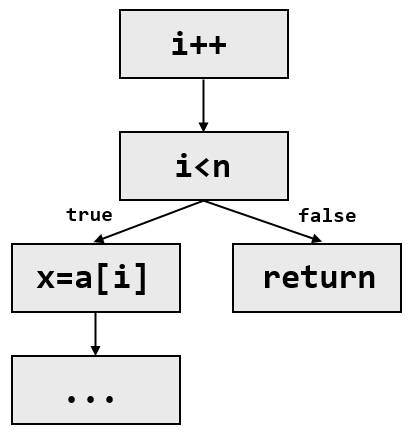
\includegraphics[width=0.3\textwidth]{images/symbolic_execution.png}
		\caption{Ausführungspfade für die symbolische Ausführung einer if-Anweisung}
\end{SCfigure}

Der aktuelle Zustand der Ausführung wird dabei durch zwei verschiedene Strukturen charakterisiert: 
Den Heap, der alle Elemente (engl. heap chunks) des Speichers beinhaltet sowie eine Liste
der geschlussfolgerten Annahmen (engl. assumptions). Bei der Ausführung der Vorbedingungen werden
diese Aussagen nun untersucht und entweder zum Heap hinzugefügt oder zu den Annahmen.

Beim Verstehen dieser Schritte ist die Verifast-Oberfläche sehr hilfreich, da sie den aktuellen
Zustand für einen beliebigen Haltepunkt anzeigen kann. Die folgende Situation zeigt die Ausführung
einer \lstinline{mismatch}-Implementierung bis zum gesetzten Haltepunkt (gelb hervorgehoben).

\begin{center}
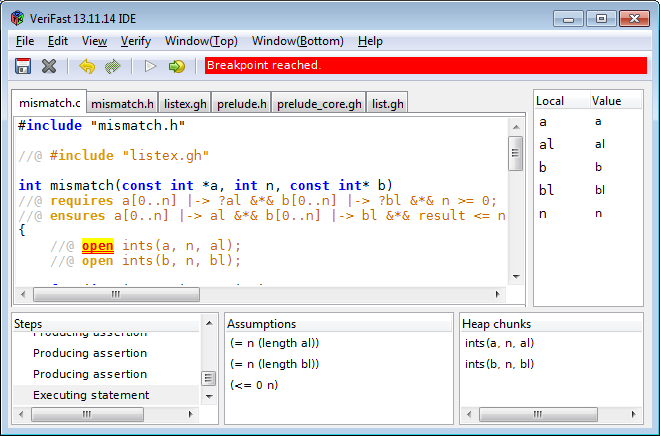
\includegraphics[width=1.0\textwidth]{images/verifast-state-after-precondition.png}
\end{center}

Gut zu erkennen ist, dass logische Ausdrücke wie \(n >= 0\) in die Liste der Annahmen 
(im Bild als \glqq Assumptions\grqq betitelt) aufgenommen wurden. Die \lstinline{ints}-Prädikate hingegen
wurden zum Heap hinzugefügt. Diesen Prozess nennt Verifast \glqq Producing assertion\grqq, wobei sich das Verb
\glqq Producing\grqq auf das Hinzufügen von Elementen zum aktuellen Zustand der symbolischen Ausführung
bezieht.

Das Gegenteil - \glqq Consuming assertion\grqq - findet z.B. beim Verifizieren der Nachbedingungen statt.
Verifast versucht dann alle erforderlichen Aussagen in der Liste der Annahmen bzw. im Heap zu finden
und diese, wenn sie denn passen, zu entfernen. Zusätzlich dazu wird am Ende einer Funktion - beim 
\glqq Leak check\grqq - auch überprüft, dass der Heap (der aktuellen Funktion) leer ist. Ist das nicht 
der Fall so wurde der entsprechende Speicher nicht korrekt bereinigt oder zumindest war Verifast nicht 
in der Lage das Gegenteil zu beweisen.

In dem Fall von mismatch würde Verifast die Heap chunks \lstinline{ints(a, n, al)} sowie
\lstinline{ints(b, n, bl)} beim Konsumieren der Nachbedingung auf dem Heap finden, entfernen und
somit erfolgreich verifizieren können, dass der Speicher so wie vor dem Aufruf vorhanden ist.



\section{Assertions und Ghost-Commands}

Zusicherungen (engl. assertions) und Ghost-Commands sind Annotationen, die direkt in den Implementierungs-Code
geschrieben werden. Assertions stellen sicher, dass der enthaltene Ausdruck wahr ist und sind ein nützliches Hilfsmittel, 
um die Verifizierung besser nachzuvollziehen als auch verständlicher zu machen. Insbesondere dann, wenn das Verifikationswerkzeug 
nicht triviale Schlüsse zieht, ist es von Vorteil Assertions zu ergänzen und im Code zu belassen.

Ghost-Commands hingegen enthalten Anweisungen für die Verifizierung, z.B. das Aufrufen anderer Sprachkonstrukte 
(z.B. Lemmata oder Fixpointfunktionen, siehe \ref{verifizierung:lemma}). Sie helfen dem Werkzeug logische Schlüsse 
zu ziehen, die es alleine nicht tun kann.
\newline
\newline
Der folgende Quellcode zeigt einen Ausschnitt aus einer rekursiven Implementierung für \lstinline{equal} und dient
hier als Anschauungsmaterial für die Erklärung der oben genannten Annotationstypen:

\lstinputlisting[language=C, caption=Rekursive Implementierung für \lstinline{equal} mit Verifast]{codes/equal_recursive_verifast.c}

Diese Implementierung zeigt nur die Abbruchbedingung der Rekursion - ist \lstinline{n == 0}, so sind die
leeren Listen gleich und die Berechnung terminiert. 

Die Zeilen 9 und 10 sind Assertions, die formal beschreiben, dass die induktiven Listen \lstinline{al} und
\lstinline{bl} die Länge 0 haben müssen und somit gleich lang sind. Damit Verifast in der Lage ist das zu
beweisen sind die zwei Ghost-Commands in Zeile 5 und 6 notwendig. Sie öffnen das \lstinline{ints}-Prädikat
und bringen somit dessen Inhalt in die Liste der Annahmen. Erst dadurch ist für Verifast ersichtlich, dass 
\lstinline{n} gleichzusetzen ist mit \texttt{length(al)} und \texttt{length(bl)}. Außerdem produziert
das Öffnen des Prädikats die Formel \lstinline{al = nil} bzw. \lstinline{bl = nil} (siehe Definition
des Prädikats in Listing 3.9 oder 4.2). Damit löst sich die Assertion \lstinline{al == bl} in den
trivialen Vergleich \lstinline{nil == nil} auf.
\newline
\newline
Das Öffnen der Prädikate konsumiert gleichzeitig auch die entsprechenden Heap-Chunks, was jedoch dazu führt,
dass diese beim Produzieren der Nachbedingung fehlen. Sie müssen also vor der \(return\)-Anweisung
wieder geschlossen werden (Zeile 11 und 12), damit sie dann wieder an den Aufrufer zurückgegeben werden können 
- so wie es die Nachbedingung verlangt.

Das Schreiben dieser \(close\)-Annotation ist jedoch oft nicht notwendig, da Verifast sie automatisch
einführt, wenn es sich um ein sogenanntes präzises Prädikat handelt. Darunter versteht Verifast Prädikate mit 
eingehenden und ausgehenden Parametern, die exakt die gleiche Speicherregion repräsentieren. 

\begin{figure}[H]
Die Kennzeichnung als präzises Prädikat geschieht über die Nutzung eines Semikolons bei der Trennung
der Prädikaten-Parameter:

\lstinputlisting[language=C, caption=Präzises Prädikat \lstinline{ints}]{codes/ints_precise_predicate_verifast.c}
\end{figure}
Präzise Prädikate versucht Verifast während der Verifizierung automatisch zu öffnen und ggf. auch zu
schließen. Dadurch ist in der obigen Implementierung das Schreiben der \texttt{close}-Anweisungen
nicht zwingend notwendig.
\newline
\newline
Assertions in ACSL werden genauso notiert wie in Verifast. Ghost-Commands hingegen werden
mit dem Schlüsseltwort \lstinline{ghost} eingeleitet, sind aber generell nicht so oft wie in
Verifast notwendig. Das kommt daher, dass Frama-C aufwendigere Berechnungen durchführt, um
entsprechende logische Schlüsse zu ziehen. Das ist jedoch auch spürbar, wenn man die
Geschwindigkeit der Werkzeuge vergleicht.


\section{Schleifeninvarianten}

Schleifeninvarianten beschreiben eine Eigenschaft, die vor und nach jeder Iteration gültig ist. Sie
werden wie Ghost-Commands per Annotation an die Schleife geschrieben und helfen dem Werkzeug die
Nachbedingungen zu verifizieren.

\begin{figure}[H]
Der folgende Quellcode zeigt eine ACSL-Implementierung für \lstinline{mismatch}
(Spezifikation siehe Listing 3.11):
\lstinputlisting[language=C, caption=Implementierung für \lstinline{mismatch} mit ACSL-Annotationen]{codes/mismatch_acsl.c}
\end{figure}

Die Invariante in Zeile 4 beschreibt den Gültigkeitsbereich der Variable \lstinline{i}, in Zeile 5 wird definiert, 
dass alle Elemente \lstinline{< i } der beiden Arrays gleich sind. Außerdem verlangt ACSL, dass alle
Variablen-Manipulationen für die Schleife explizit angegeben werden (siehe Zeile 6). Damit kann das Werkzeug
nun die beiden Fälle aus den Nachbedingungen beweisen.

Hier erweist es sich auch wieder als vorteilhaft, dass für die Spezifikation bereits das Prädikat
\lstinline{IsEqual} definiert wurde, denn in der Schleifeninvariante kann dieses wiederverwendet werden. Damit
ist auch für den Leser schneller ersichtlich, dass die Invariante beim Beweis der Spezifikation hilft.

\begin{figure}[H]
	\centering
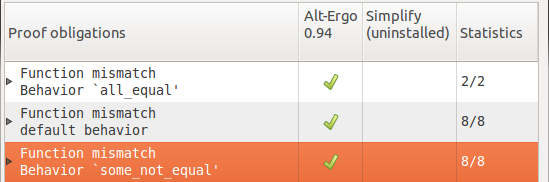
\includegraphics[width=0.8\textwidth]{images/acsl-prove-mismatch.png}

Die Implementierung für \lstinline{mismatch} wurde erfolgreich verifiziert.
\end{figure}

Invarianten in ACSL und Verifast funktionieren bis auf kleinere syntaktische Unterschiede nach dem gleichen Prinzip.
Wie schon von den Spezifikationen bekannt, ist es auch hier in Verifast wieder notwendig die Invarianten in nur
einer einzigen Annotation auszudrücken. Außerdem kann der Schleifenkörper nur auf Heap-Chunks zurückgreifen, die
in der Invariante explizit angegeben werden. Verifast entfernt vor dem Schleifenbeginn alle aktuellen Chunks
und stellt diese nach dem Austritt aus der Schleife wieder her. Der Schleifenkörper verhält sich also
wie eine eigenständige Funktion.

\begin{figure}[H]
Nachfolgend ist die Implementation von oben nochmal gezeigt, an der Stelle aber mit Invarianten für Verifast.

\lstinputlisting[language=C, caption=Implementierung für \lstinline{mismatch} mit Verifast-Annotationen]{codes/mismatch_verifast.c}
\end{figure} 

Wie in der dazugehörigen Spezifikation (siehe Listing 3.10) wird die Funktion \lstinline{take} genutzt,
um die ersten \lstinline{i} Elemente der Liste \lstinline{al} und \lstinline{bl} zu vergleichen.
Die Einschränkung des Wertebereichs der Variablen \lstinline{i} ist identisch mit der ACSL-Variante -
bis auf den syntaktischen Unterschied, dass Verifast keine Verkettung von Vergleichsoperatoren erlaubt.

Wie oben beschrieben muss außerdem der Speicherinhalt der Arrays \lstinline{al} und \lstinline{bl} für
den Schleifenkörper zugreifbar gemacht werden. Deshalb finden sich hier die \lstinline{ints}-Prädikate
aus der Spezifikation wieder. Sie stellen sicher, dass die Elemente \lstinline{a[0 <= i < n]} gelesen
werden können.

Im Unterschied zu Verifast ist es nicht notwendig und auch nicht möglich Schreibrechte für die lokale Variable 
\lstinline{i} zu erteilen. Auf lokale Variablen darf der Schleifenkörper in Verifast immer zugreifen, lesend
als auch schreibend.
\newline
\newline
Versucht man die Implementierung mit Verifast nun zu beweisen, erhält man einen Fehler: Die Schleifeninvariante
konnte nicht bewiesen werden. 
Das liegt daran, dass das Werkzeug aus dem Schleifenkörper allein nicht folgern kann, dass in der nächsten Iteration 
die Länge der gleichen Listen um eins gewachsen ist. Der Fehler tritt darum beim \lstinline{==} der Invariante auf.
Zur Lösung wird ein Lemma benötigt, welchen diesen Schritt für Verifast nachvollziehbar macht.

\section{Lemmata und Axiome}
\label{verifizierung:lemma}

Lemmata sind Funktionen, die dem Werkzeug helfen sollen logische Schritte zu machen. Wie normale
Funktionen besitzen sie Vorbedingungen sowie Nachbedingungen und müssen explizit aufgerufen werden.
Da es sich um Code handelt, der nur für das Verifikationswerkzeug bestimmt ist, findet der Aufruf
in einem Ghost-Command per Annotation statt:

\lstset{frame=none, numbers=none}                      
\begin{lstlisting}
//@ ghost take_plus_one(i, al);
\end{lstlisting}
\lstset{frame=single, numbers=left}    
Das Lemma \lstinline{take_plus_one} sorgt dafür, dass Verifast den Ausdruck \lstinline{take(i + 1, al)}
versteht und die Invariante (siehe Listing 4.4 oben) vollständig beweisen kann. Es ist wie folgt
definiert (in der von Verifast mitgelieferten listex.gh):
\begin{figure}[H]
\lstinputlisting[language=C, caption=Lemma \lstinline{take_plus_one}]{codes/take_plus_one.c}
\end{figure}
Wird dieses Lemma in obiger Schleife (nach dem if-Block) aufgerufen, so kann Verifast
die Invariante \lstinline{take(i, al) == take(i, bl)} nach dem Induktionsschritt \lstinline{i++}
beweisen. Der folgende Code zeigt den Aufruf des Lemmas innerhalb der Schleife plus weitere Assertions:
\begin{itemize}
\item Zeile 8 folgt aus der Invariante selbst
\item Zeile 9 ist die Schlussfolgerung aus der vorangegangenen if-Anweisung
\item Zeilen 10 und 11 wenden das Lemma auf die Listen \lstinline{al} und \lstinline{bl} an
\item Zeilen 12 und 13 beschreiben den Effekt (die Nachbedingung) des Lemmas
\item Zeile 14 inkremniert die Schleifenvariable (verschoben aus Schleifenkopf, da ansonsten die folgende Zusicherung nicht im Code platziert werden kann)
\item Zeile 15 stellt die nun bewiesene Invariante dar
\end{itemize}

\lstinputlisting[language=C, firstline=3, lastline=18, caption=Aufruf Lemma \lstinline{take_plus_one} in Schleife]{codes/mismatch_verifast_2.c}

Es besteht in Verifast auch die Möglichkeit ein Lemma mit dem Schlüsselwort \lstinline{lemma_auto} zu deklarieren.
Damit muss es nicht mehr explizit aufgerufen werden, sondern wird automatisch genutzt, wie die von 
ACSL bekannten Axiome. Richtig dokumentiert ist diese Funktionalität allerdings nicht, da sie laut den Verifast-Autoren
nur für Experten gedacht ist. \todo{referenz auf paper von bart jacobs}

Ein Grund dafür ist, dass eine unbedachte Ausnutzung des Schlüsselwortes
den von Verifast genutzten SMT-Solver (Satisfability Modulo Theories) in eine Endloschleife bringen kann. Ein
weiterer Nachteil ist zudem, dass der Verifikationsprozess nicht mehr vollständig nachvollziehbar ist.
Denn den automatischen Aufruf des Lemmas zeigt Verifast nicht an, wenn man die einzelnen
Schritte des symbolischen Ausführungspfades auf der Oberfläche inspiziert.
\newline
\newline
Ein sinnvoller Einsatz der automatischen Lemmata sind globale Invarianten, z.B. die Eigenschaften von Datenstrukturen
im C- oder Ghostcode. In ACSL gibt es für diese Fälle die sogenannten Typ-Invarianten, die entweder zu jeder Zeit oder
nur beim Ein- und Austritt in eine Methode gelten müssen. Letztere werden als schwachte Invarianten bezeichnet.

Tatsächlich wurde bei der Verifizierung der gezeigten Implementierungungen bereits eine solche
globale Invariante - formuliert als Lemma - automatisch genutzt. Die Funktion \lstinline{ints_inv}
(definiert in prelude.h) beschreibt den Zusammenhang zwischen der Fixpunktfunktion \texttt{length}
(Länge einer Liste) und dem \lstinline{ints}-Prädikat:

\lstinputlisting[language=C, caption=Lemma \lstinline{ints_inv}]{codes/ints_inv.c}

Ohne dieses Lemma wäre die Verifizierung der \lstinline{mismatch}-Implementierung (Listing 4.4)
nicht erfolgreich, da die Information fehlen würde, dass \lstinline{n} (im Lemma \lstinline{count})
der Länge der Listen entspricht.
\newline
\newline
Analog zu den Axiomen in ACSL ist es auch in Verifast nicht notwendig einen Beweis der Lemmata anzugeben -
das Werkzeug vertraut den Angaben blind. Dort wo es jedoch möglich ist, sollte man einen Beweis anführen,
damit die Verifizierung keine Schwachstellen besitzt.
Der Beweis wird als Funktionskörper definiert und automatisch geprüft. Verifast testet außerdem die
Terminierung der Lemmafunkton. 
Dabei muss \todo{zitat zu tutorial, seite 15} darauf geachtet werden, dass das Werkzeug die Induktion auch 
erkennen kann. Für die Induktion über eine Liste ist es beispielsweise notwendig den Beweis mit einer 
\texttt{switch}-Anweisung zu beginnen. Eine semantisch äquivalente Form mit \texttt{if}-Anweisungen wird 
nicht unterstützt.
\begin{figure}[H]
Der folgende Ghost-Code zeigt den Beweis des entsprechenden Lemmas. Um das Verstehen zu erleichtern,
wurden Assertions eingefügt.
\lstinputlisting[language=C, caption=Beweis des Lemmas \lstinline{take_one_plus}]{codes/take_plus_one_proof.c}
\end{figure} 
Für viele in Verifast enthaltene Lemmata gibt es bereits Beweise. Diese befinden sich jedoch in einer separaten
Datei, damit das Werkzeug nicht bei jeder Verifizierung all diese nachprüfen muss.

\section{Terminierung}

Um die totale Korrektheit zu beweisen, ist es notwendig die Terminierung der Implementierung zu
verifizieren. Im Falle von Schleifen, muss eine sogenannte Variante ergänzt werden, die
in jeder Iteration kleiner wird und in endlich Schritten zu einem kleinstem Element führt.

Beide Verifikationswerkzeuge erlauben die Notation und Verifizierung einer solchen Variante analog zur
Schleifeninvariante. Die folgende Schleife (aus der \texttt{equal}-Implementierung) wurde mit einer Variante 
in ACSL-Syntax angereichert. Dieselbe Variante für Verifast würde genauso lauten, allerdings
mit dem Schlüsselwort \texttt{decreases} eingeleitet werden.
\begin{figure}[H]
\lstinputlisting[language=C, caption=Schleifenvariante in ACSL]{codes/loop_variant_acsl.c}
\end{figure}

Tatsächlich kann bereits ein kleiner Tippfehler dafür sorgen, dass die Implementierung
nicht terminiert. Das Werkzeug Verifast beweist die funktionale Korrektheit aber trotzdem
(siehe Screenshot). Frama-C dagegen warnt wenn eine Variante fehlt und generiert selbstständig
eine Dummy-Variante. So fällt zumindest auf, dass die Terminierung noch nicht bewiesen ist.

\begin{figure}[H]
	\centering
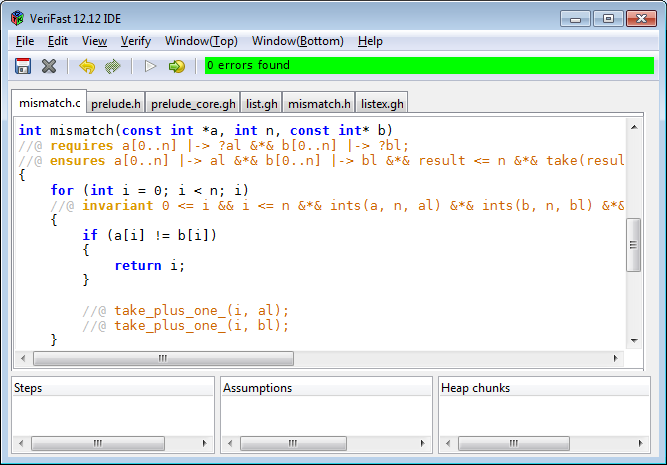
\includegraphics[width=1.0\textwidth]{images/verifast-partial-correctness.png}
\caption{Tippfehler beim \texttt{i++} in der Implementierung}
\end{figure}

Das Beispiel zeigt, dass automatische Tests an dieser Stelle einen wichtigen Beitrag leisten
können. Denn ein einfacher Unit-Test würde reichen, um den Tippfehler aufzudecken. In allen
Fällen in denen die Terminierung nur sehr schwierig oder gar nicht zu beweisen ist, bieten
Unit-Tests außerdem eine einfachere bzw. überhaupt eine Lösung. Auch wenn damit natürlich
kein Beweis der totalen Korrektheit zu erbringen ist.
\newline
\newline
ACSL kann darüber hinaus auch die Terminierung von rekursiven Funktionen prüfen, was in
Verifast derzeit nicht möglich ist.


\section{Überläufe erkennen}

overflow checken

\section{Speicherprobleme aufdecken}

malloc/free - chunks

zeigen an hand von main-funktion (unit-test)

verifast hilft klar zu dokumentieren wer für speicher verantwortlich ist (rufer oder gerufener)


